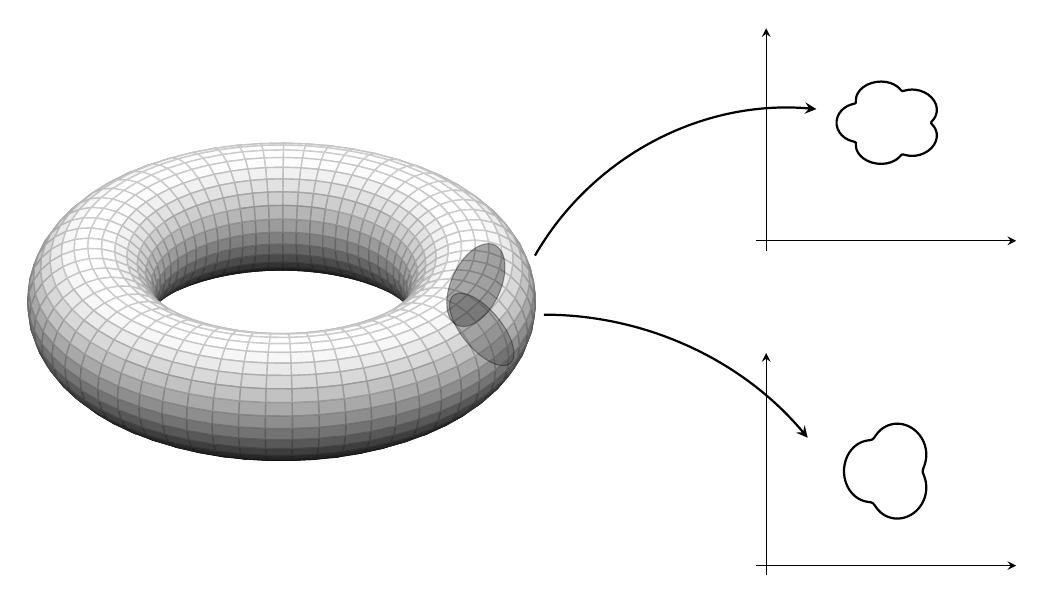
\begin{tikzpicture}[scale=1.25]
\shorthandoff{>}
\pgfplotsset{compat=1.6}
%
\pgfmathsetmacro\a{3} % rayon de rotation du centre du cercle definissant le tore
\pgfmathsetmacro\r{1} % rayon du cercle definissant le tore
%
\pgfmathsetmacro\au{.25} % 1/2 grand axe ellipse 1
\pgfmathsetmacro\bu{.45} % 1/2 petit axe ellipse 1
\pgfmathsetmacro\tu{25} % angle de rotation ellipse 1
%
\pgfmathsetmacro\ad{.2} % 1/2 grand axe ellipse 2
\pgfmathsetmacro\bd{.45} % 1/2 petit axe ellipse 2
\pgfmathsetmacro\td{-40} % angle de rotation ellipse 2
%
\pgfmathsetmacro\ru{.08} % rayon epitrocoide 1
\pgfmathsetmacro\ku{5} % ku-epicicotroide
\pgfmathsetmacro\du{.7} % \du*\ru = distance du point au centre (du = 1: epicicloide)
%
\pgfmathsetmacro\rd{.1} % rayon epitrocoide 2
\pgfmathsetmacro\kd{3} % ku-epicicotroide
\pgfmathsetmacro\dd{.6} % \du*\ru = distance du point au centre (du = 1: epicicloide) 
%
%
% Trace du domaine (tore)
% -----------------------------
%
\begin{axis}[axis equal image , clip=false , axis lines = none , colormap/blackwhite]
%y dir=reverse,
%axis on top
%
% Tore:
%view={45}{45}
\addplot3[domain = 0:360 , y domain = 0:360 , samples = 30 , samples y = 60 , surf , z buffer = sort]
({(\a+\r*cos(x))*sin(y)} , {(\a+\r*cos(x))*cos(y)} , {\r*sin(x)}); % ecuacion del tore
\end{axis}
%
% Ellipse 1
\filldraw[domain = 0:360 , samples=50 , fill = black , opacity = .35] plot 
({1.8*\a+\au*cos(\x)*cos(\tu)+\bu*sin(\x)*sin(\tu)} ,
  {.85*\a-\au*cos(\x)*sin(\tu)+\bu*sin(\x)*cos(\tu)});
%
% Ellipse 2
\filldraw[domain = 0:360 , samples=50 , fill = black!75 , opacity = .35] plot 
({1.82*\a+\ad*cos(\x)*cos(\td)+\bd*sin(\x)*sin(\td)} ,
  {.7*\a-\ad*cos(\x)*sin(\td)+\bd*sin(\x)*cos(\td)});
%
%
% Premier depliement
%
\draw[thick , domain = 0:360 , samples = 100 , yscale = .8] plot(
{3.2*\a+\ru*((\ku+1)*cos(\x)-\du*cos((\ku+1)*\x))} ,
{1.75*\a+\ru*((\ku+1)*sin(\x)-\du*sin((\ku+1)*\x))});
%
\draw[thick , >=stealth , ->]  ({2*\a},{.95*\a}) arc (150:85:3) ;
\draw[>=stealth , ->]  ({2.75*\a},{\a}) -- ({2.75*\a+5.5*\ru*(\ku+1)},{\a});
\draw[>=stealth , ->]  ({2.75*\a+.1},{\a-.1}) -- ({2.75*\a+.1},{\a+4.5*\ru*(\ku+1)});
%
%
% Second depliement
%
\draw[thick , domain = 0:360 , samples = 100 , yscale = 1.1] plot(
{3.2*\a+\rd*((\kd+1)*cos(\x)-\dd*cos((\kd+1)*\x))} ,
 {.2*\a+\rd*((\kd+1)*sin(\x)-\dd*sin((\kd+1)*\x))});
%
\draw[thick , >=stealth , ->]  ({2.03*\a},{.75*\a}) arc (90:40:3.5) ;
\draw[>=stealth , ->]  ({2.75*\a},{-.1*\a}) -- ({2.75*\a+5.5*\ru*(\ku+1)},{-.1*\a});
\draw[>=stealth , ->]  ({2.75*\a+.1},{-.1*\a-.1}) -- ({2.75*\a+.1},{-.1*\a+4.5*\ru*(\ku+1)});
\end{tikzpicture}
